% Options for packages loaded elsewhere
\PassOptionsToPackage{unicode}{hyperref}
\PassOptionsToPackage{hyphens}{url}
\documentclass[
]{article}
\usepackage{xcolor}
\usepackage{amsmath,amssymb}
\setcounter{secnumdepth}{-\maxdimen} % remove section numbering
\usepackage{iftex}
\ifPDFTeX
  \usepackage[T1]{fontenc}
  \usepackage[utf8]{inputenc}
  \usepackage{textcomp} % provide euro and other symbols
\else % if luatex or xetex
  \usepackage{unicode-math} % this also loads fontspec
  \defaultfontfeatures{Scale=MatchLowercase}
  \defaultfontfeatures[\rmfamily]{Ligatures=TeX,Scale=1}
\fi
\usepackage{lmodern}
\ifPDFTeX\else
  % xetex/luatex font selection
  \setmainfont{Times New Roman}
\fi
\usepackage[letterpaper,left=1in,right=1in,top=0.9in,bottom=0.8in]{geometry}
\linespread{1.1}
% Use upquote if available, for straight quotes in verbatim environments
\IfFileExists{upquote.sty}{\usepackage{upquote}}{}
\IfFileExists{microtype.sty}{% use microtype if available
  \usepackage[]{microtype}
  \UseMicrotypeSet[protrusion]{basicmath} % disable protrusion for tt fonts
}{}
\makeatletter
\@ifundefined{KOMAClassName}{% if non-KOMA class
  \IfFileExists{parskip.sty}{%
    \usepackage{parskip}
  }{% else
    \setlength{\parindent}{0pt}
    \setlength{\parskip}{6pt plus 2pt minus 1pt}}
}{% if KOMA class
  \KOMAoptions{parskip=half}}
\makeatother
\usepackage{longtable,booktabs,array}
\newcounter{none} % for unnumbered tables
\usepackage{calc} % for calculating minipage widths
% Correct order of tables after \paragraph or \subparagraph
\usepackage{etoolbox}
\makeatletter
\patchcmd\longtable{\par}{\if@noskipsec\mbox{}\fi\par}{}{}
\makeatother
% Allow footnotes in longtable head/foot
\IfFileExists{footnotehyper.sty}{\usepackage{footnotehyper}}{\usepackage{footnote}}
\makesavenoteenv{longtable}
\usepackage{graphicx}
\makeatletter
\newsavebox\pandoc@box
\newcommand*\pandocbounded[1]{% scales image to fit in text height/width
  \sbox\pandoc@box{#1}%
  \Gscale@div\@tempa{\textheight}{\dimexpr\ht\pandoc@box+\dp\pandoc@box\relax}%
  \Gscale@div\@tempb{\linewidth}{\wd\pandoc@box}%
  \ifdim\@tempb\p@<\@tempa\p@\let\@tempa\@tempb\fi% select the smaller of both
  \ifdim\@tempa\p@<\p@\scalebox{\@tempa}{\usebox\pandoc@box}%
  \else\usebox{\pandoc@box}%
  \fi%
}
% Set default figure placement to htbp
\def\fps@figure{htbp}
\makeatother
\setlength{\emergencystretch}{3em} % prevent overfull lines
\providecommand{\tightlist}{%
  \setlength{\itemsep}{0pt}\setlength{\parskip}{0pt}}
\usepackage{bookmark}
\IfFileExists{xurl.sty}{\usepackage{xurl}}{} % add URL line breaks if available
\urlstyle{same}
\hypersetup{
  pdftitle={Regulatory Resilience in Technology Transfer Systems: Relational Contracting and State Capacity in Vietnam},
  hidelinks,
  pdfcreator={LaTeX via pandoc}}

\title{Regulatory Resilience in Technology Transfer Systems: Relational
Contracting and State Capacity in Vietnam}
\author{}
\date{}

\begin{document}
\maketitle

\emph{Anonymous manuscript for The Journal of Technology Transfer}

\section{Abstract}\label{abstract}

Technology transfer succeeds when a continuing inter-organisational
relationship reaches operating capability while remaining connected to
multiple public mandates. This article develops a dual-function account
of the technology-transfer contract: it is both a private performance
arrangement and a compliance protocol that organises information and
regulatory engagement without altering public powers.
Vietnam\textquotesingle s 2025--2026 reforms provide a theory-informing
case. A systematic qualitative analysis of thirty-four Vietnamese
policy, professional and legal publications identifies recurring
transaction problems; two source-traced vignettes expose their temporal
and organisational structure. Doctrinal analysis then tests those
problems against technology-transfer, intellectual-property,
competition, data, artificial-intelligence and sectoral law. The
analysis identifies three connected mechanisms: verifiable delivery and
adaptation, cross-regime compliance coordination, and complementary
administrative and industrial capability. The statutory framework
provides extensive but distributed protection. It does not, however,
supply a technology-specific default connecting acceptance, corrective
work, payment and warranty, or a routine interface through which firms
can obtain coordinated, reviewable regulatory answers. Relational
contracting and state capacity are therefore complements: their
interaction produces regulatory resilience, which in turn supports
transfer performance. A time-limited coordination pilot and two
propositions make that causal argument testable. Supplementary
text-model diagnostics are retained only as an audit of theme
sensitivity, not as statistical evidence from the small corpus. The
contribution is a mechanism-based account of regulatory resilience that
can be examined beyond Vietnam.

\textbf{Keywords:} technology transfer; regulatory resilience;
relational contracts; state capacity; administrative coordination;
Vietnam

\textbf{JEL codes:} O31; O32; O38; K12; K21

\section{1 Introduction}\label{introduction}

Technology transfer is often described as a movement of knowledge or
rights from one organisation to another. In practice, the movement is
rarely complete at signature. Operating capability may depend on
training, trial production, corrective work, access to tacit know-how
and repeated decisions about adaptation. The same transaction may also
engage intellectual-property, competition, data,
artificial-intelligence, investment and sectoral rules. A transfer
system is therefore resilient only when it can sustain private
performance and connect the transaction to applicable public mandates as
technologies and circumstances change.

This problem is especially visible in economies that seek advanced
technology while rebuilding their legal and administrative architecture.
It is tempting to diagnose every overlap as fragmentation or every
missing technology-specific rule as a regulatory void. That diagnosis is
too quick. Specialisation across statutes can preserve expertise and
accountability, and general private law can supply remedies where a
dedicated transfer statute is silent. The analytically useful question
is narrower: which connections are needed for a continuing transfer
relationship to reach demonstrable operating capability, and which of
those connections are supplied by law, contract or administrative
practice?

Vietnam provides a theory-informing case rather than a representative
case of all emerging economies. It combines a dedicated Law on
Technology Transfer with general contract law, intellectual-property and
competition regimes, and recently enacted rules on data, artificial
intelligence, digital industries and high technology. Between 2025 and
2026 the legislature expanded the objects of transfer, revised
intellectual-property rules, enacted a national artificial-intelligence
statute, adopted semiconductor provisions and replaced the principal
technology-transfer decree. The reforms make it possible to observe how
new sectoral regimes interact with an older contract architecture.

The article begins with published accounts rather than presumed
statutory omissions. A systematic qualitative document analysis
organises a bounded corpus of thirty-four Vietnamese publications by
source type, transaction problem and institutional function. The
documents identify questions; they do not establish population
frequencies, causal effects or the prevalence of defective contracts.
Doctrinal analysis then asks where the operative answer to each question
is located, under what conditions it applies and whether a tailored
default or connection remains unspecified. This sequence preserves the
distinct evidential roles of documentary interpretation and legal
analysis.

Three research questions guide the study. First, which performance,
compliance and capability questions emerge from the principal themes in
the selected discourse? Second, which Vietnamese rules answer those
questions, and where does the review identify no tailored default or
routine regulatory connection? Third, what does the resulting pattern
imply for the resilience of technology-transfer systems and for
subsequent empirical evaluation?

The central contribution is a dual-function account of the
technology-transfer contract. The contract organises delivery,
acceptance, training, adaptation and payment between private parties. It
can also organise the records, information duties, role allocation and
cooperation needed to engage public authorities. The second function
does not make regulators parties to the contract or permit private
agreement to alter mandatory duties. It treats the transaction record as
connective infrastructure between distinct legal functions.

The analysis identifies three mechanisms. The first is verifiable
performance over time: a transfer must connect demonstrable delivery to
correction, payment and warranty. The second is cross-regime compliance
coordination: recognising an algorithm or dataset as transferable does
not determine ownership, lawful access, security duties or downstream AI
responsibilities. The third is complementary capability: access to a
patent or model cannot substitute for skills, facilities, finance,
valuation expertise or administrative delivery. These mechanisms explain
why more detailed documentation can be necessary without being
sufficient.

The article proceeds as follows. Section 2 develops the theoretical
framework and contribution. Section 3 explains the qualitative document
analysis, supplementary audit and doctrinal scope. Section 4 presents
the three mechanisms through an evidence matrix and source-traced
vignettes. Section 5 states the dual-function framework and a
coordination pilot. Section 6 discusses transferability, rival
explanations and testable implications. Section 7 concludes.

\section{2 Theory and contribution}\label{theory-and-contribution}

Relational contract theory directs attention from isolated promises to
continuing cooperation. Macaulay (1963) showed that business exchange
relies on practices and relationships that exceed formal terms. Macneil
(1980) treated contractual obligations as embedded in continuing social
relations. Williamson (1979) offered a distinct transaction-cost
explanation in which uncertainty and transaction-specific investment
create governance problems after parties commit resources. These
approaches should not be collapsed, but together they identify
adaptation, information exchange and safeguards against opportunism as
central to transactions whose performance cannot be specified completely
in advance.

Innovation contracting sharpens that insight. Gilson, Sabel and Scott
(2009) explain how formal arrangements can support iterative
collaboration rather than simply define a finished product. A detailed
document and a well-governed relationship are not alternatives. The
relevant question is which provisions make experimentation, verification
and correction workable. For technology transfer, that includes
specifications of operating capability, access to tacit knowledge,
training deliverables, testing responsibilities, change procedures and
independent expert determination.

Evidence accumulated since that contribution reinforces a complementary
rather than substitutive view. Cao and Lumineau\textquotesingle s (2015)
meta-analysis of 149 studies finds that contractual governance is
positively associated with trust and relational norms and that the
mechanisms jointly improve relationship performance. Recent work on
academic engagement likewise treats knowledge exchange as
organisationally broader than licensing and patenting (Perkmann et al.
2021). The implication for technology transfer is not that every
contingency should be specified ex ante, but that formal records and
relational routines should be designed to support learning and
adaptation together.

The innovation literature also prevents an exclusively contractual
account. Teece (1986) links returns from innovation to appropriability
and complementary assets. Grindley and Teece (1997) show the importance
of negotiated licensing and cross-licensing in semiconductors and
electronics. Bradley, Hayter and Link (2013) criticise linear accounts
of university technology transfer that neglect informal mechanisms and
organisational conditions. Bozeman (2000) and Bozeman, Rimes and Youtie
(2015) similarly treat transfer effectiveness as contingent on the
actors, objects, mechanisms and public values involved. Clear rights may
therefore be necessary without being sufficient where skills, finance,
facilities or organisational incentives remain binding constraints.

Administrative capacity connects these private relationships to public
organisation. Lodge and Wegrich (2014) distinguish analytical,
coordination, regulatory and delivery capacities. Applied to technology
transfer, those capacities concern identifying a
transaction\textquotesingle s legal implications, connecting competent
bodies, exercising lawful oversight and supporting implementation. The
presence of several statutes or authorities does not prove dysfunctional
fragmentation. Regulatory distribution becomes problematic when relevant
decisions, information or responsibilities cannot be connected in a
manner that permits lawful performance.

This systems perspective is consistent with recent technology-transfer
research. A forty-five-year review of The Journal of Technology Transfer
identifies capacity, sustainable transfer and changing non-market
environments as important directions (Abid, Cunningham and Perea-Vicente
2025). A complementary review of 1,944 university-technology-transfer
studies shows that processes, enablers and capacity now occupy a central
position in the literature (Cunningham, Menter and Starke 2025).
Together, these studies explain why a contract-only or university-only
account is incomplete: transfer outcomes depend on relationships among
firms, intermediaries, public bodies and complementary resources at
micro, meso and macro levels.

The article joins these literatures by treating regulatory resilience as
a property of connections rather than rule density. A resilient transfer
system must preserve the expertise and accountability of specialised
regimes while making their interfaces usable for the transaction.
Private performance and public compliance remain legally distinct, yet
they may depend on shared records, timely role identification and
coordinated responses. The proposed dual-function contract is one
possible connective device; an inter-agency case protocol is another.

Figure 1 states the causal architecture. Relational contracting reduces
transaction-level uncertainty by making delivery, adaptation and
information exchange workable. State capacity supplies analytical,
coordination, regulatory and delivery functions. Their interaction
creates regulatory resilience: usable connections across private
performance and public mandates. Regulatory resilience should improve
the probability that a transfer reaches operating capability, subject to
technological complexity, absorptive capacity and institutional
resources. A contract cannot bind a regulator, waive statutory powers or
privately negotiate away public duties.

The legal contribution is a scoped map of Vietnamese technology-transfer
protection after the 2025--2026 reforms. Industrial-property and
competition rules overlap more than a registration-plus-dominance
account implies; digital transfers require coordination among transfer,
data and AI statutes rather than a single ownership rule; and
technology-specific defaults for acceptance and improvements to
unregistered know-how remain unspecified in the dedicated contract
chapter. The theoretical contribution is the proposed connection between
relational performance and administrative coordination.

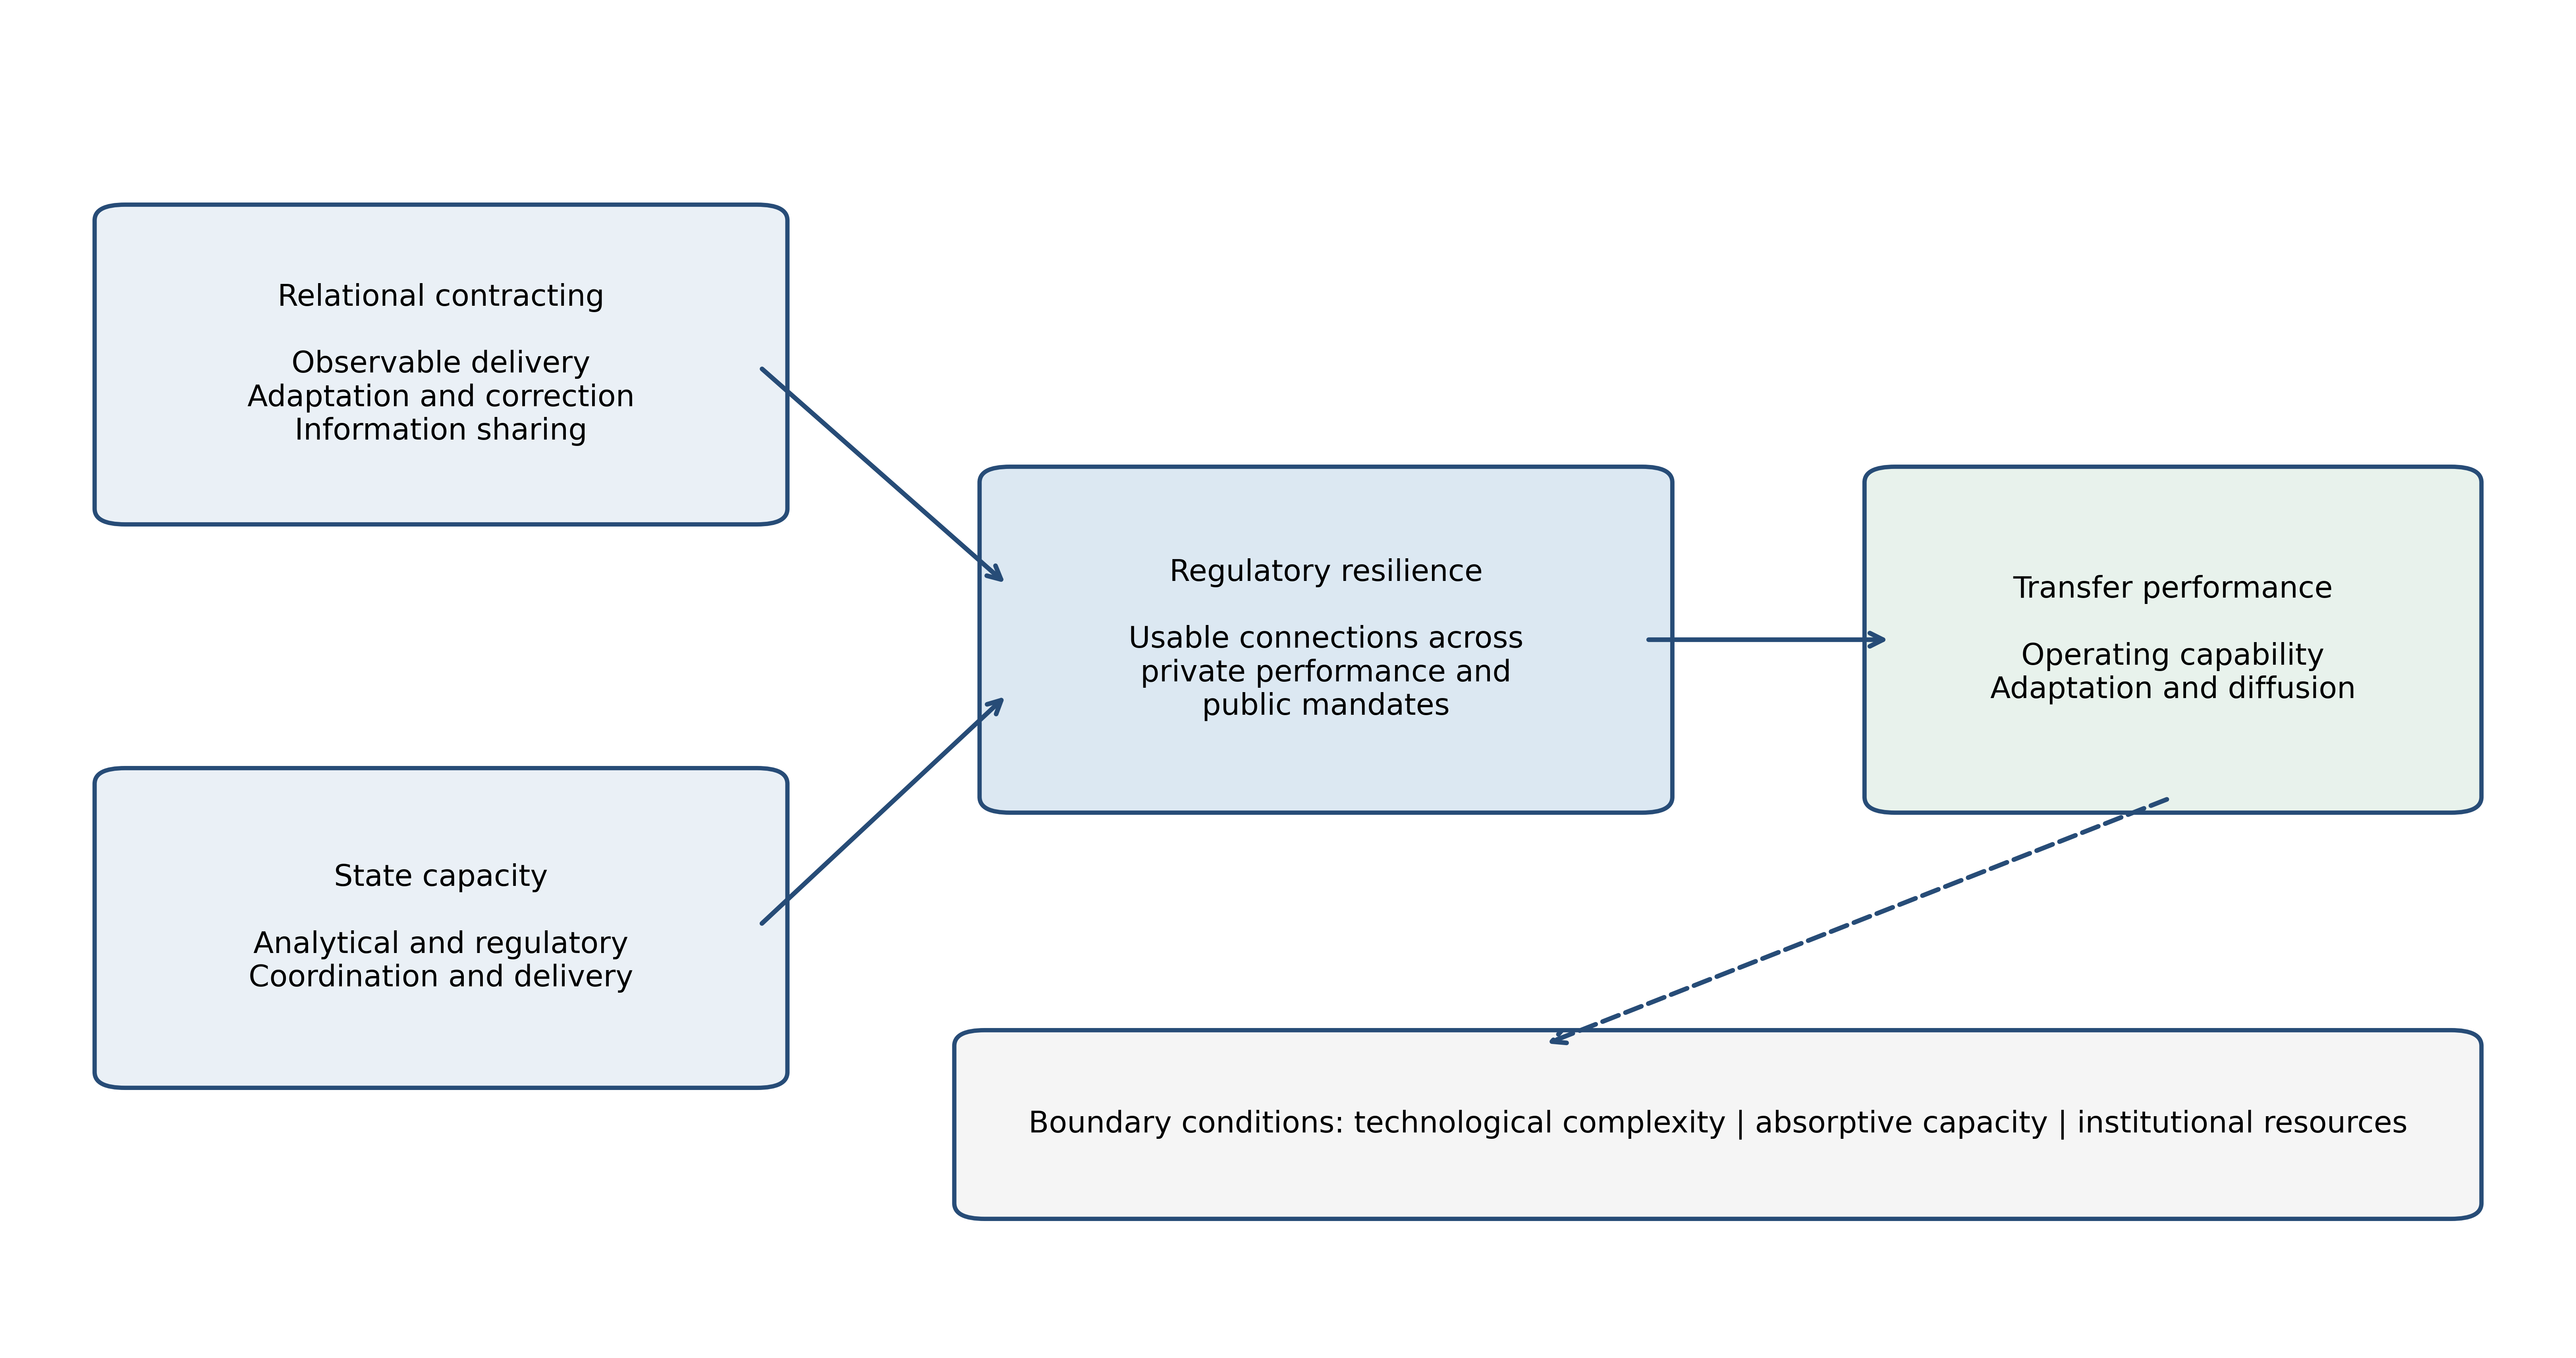
\includegraphics[width=6.3in,height=3.32141in]{figures/Fig1_Theoretical_Framework.png}

\emph{Fig. 1 Causal framework for regulatory resilience and
technology-transfer performance}

\section{3 Research design}\label{research-design}

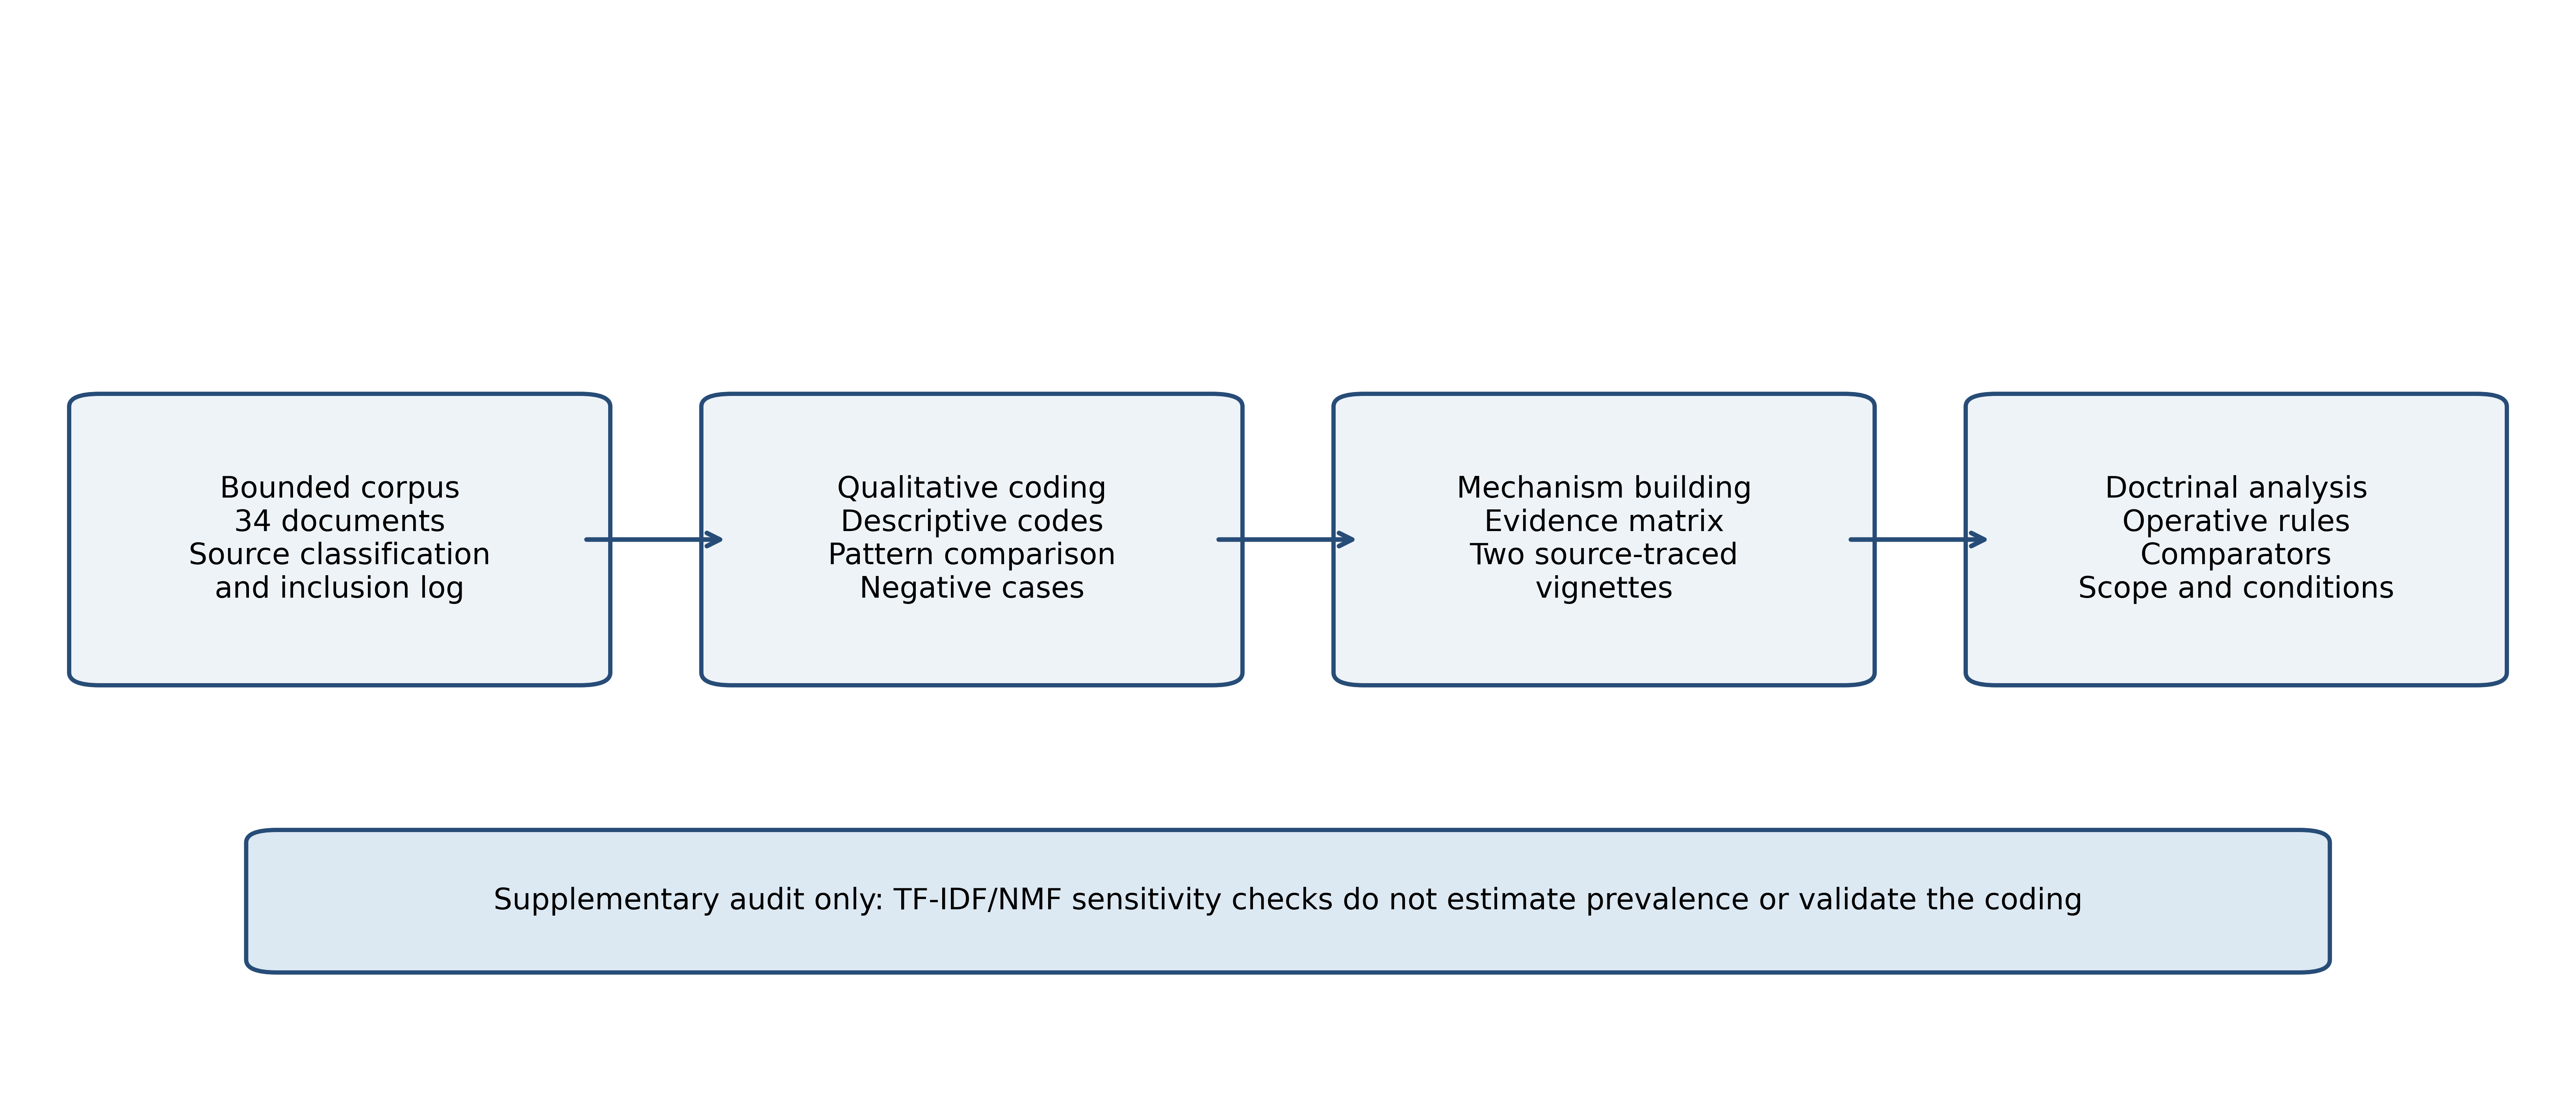
\includegraphics[width=6.4in,height=2.75963in]{figures/Fig2_Research_Design.png}

\emph{Fig. 2 Research design and evidence boundary}

\subsection{3.1 Evidence strategy and
limits}\label{evidence-strategy-and-limits}

The study uses systematic qualitative document analysis to connect
observed transaction problems to doctrinal questions. The design
separates four operations: corpus construction and source
classification; descriptive coding of the problem each passage reports;
pattern coding into candidate mechanisms; and legal assessment against
operative instruments. This separation matters because published claims
are evidence of discourse and reported experience, whereas legal
conclusions must rest on the text, scope and commencement of applicable
rules.

The coding frame was both deductive and inductive. Initial sensitising
categories came from relational contracting and state-capacity theory:
performance, adaptation, information, regulatory coordination and
complementary capability. Close reading then added object-specific codes
for acceptance, tacit know-how, restrictive licensing, data access, AI
roles, valuation, semiconductor capability and agricultural diffusion.
Pattern comparison consolidated those codes into three mechanisms only
when the same functional problem appeared across more than one source
type or legal interface. Table 2 preserves representative
source-to-inference links and a negative or limiting case for each
mechanism.

The corpus contains published discussion rather than contracts,
judgments or administrative case files. It cannot estimate prevalence,
establish causal effects or verify the outcome of a reported dispute.
The two vignettes in Section 4 are therefore source-traced
illustrations, not adjudicated case studies. No claim of theoretical
saturation or inter-coder reliability is made. The anonymized inventory,
evidence matrix and supplementary sensitivity outputs permit an audit of
selection and interpretation.

Generative AI tools assisted language editing, document restructuring
and code review. The authors independently verified the legal sources,
qualitative coding, supplementary outputs, analysis and conclusions and
retain full responsibility for the final manuscript. No AI system is
listed as an author.

\subsection{3.2 Corpus selection and qualitative
procedure}\label{corpus-selection-and-qualitative-procedure}

The bounded corpus comprises thirty-four Vietnamese-language documents
on technology transfer, science, technology and innovation. Twenty-seven
are government, policy or news publications and seven are legal or
professional analyses. Documents were included when their principal
subject was technology transfer or when they described a concrete
transfer setting in AI, semiconductors, agriculture, energy or
university research. Duplicative items were retained only when they
represented a distinct institutional voice or application setting. The
inventory records the filename and operational genre classification;
full texts remain in the research archive because most are third-party
copyrighted materials.

Table 1 reports the corpus taxonomy rather than topic-model clusters.
First-cycle coding recorded the transfer object, actor, reported
problem, institutional level and legal interface. Second-cycle
comparison asked whether the passage concerned observable performance
over time, a connection among regulatory regimes, or a complementary
capability needed to use the technology. A passage could support more
than one code, but a mechanism was retained only where the distinction
changed the relevant legal or policy response.

Validity rests on source tracing, triangulation and explicit limits
rather than statistical fit. Contract-performance claims were checked
against the dedicated statute and general private-law routes; digital
claims were checked across transfer, intellectual-property, data and AI
rules; capability claims were checked against sectoral and
administrative instruments. Contrary evidence was retained: the
existence of substantial general remedies limits any claim of a legal
vacuum, while genre sensitivity shows that contract-law concerns are
concentrated in professional sources rather than the broader policy
discourse.

Text modelling is confined to the Supplementary Information as a
sensitivity audit. On this small mixed-genre corpus, NMF, K-means and
the K scan cannot support population inference or validate the
qualitative coding. Their limited use is to show that the
contract-and-dispute vocabulary survives removal of one legal article
but disappears from a news-only model. The result supports a genre
warning, not a quantitative finding. The former MDS plot has therefore
been removed from the manuscript.

\clearpage

{\def\LTcaptype{none} % do not increment counter
\begin{longtable}[]{@{}
  >{\raggedright\arraybackslash}p{(\linewidth - 6\tabcolsep) * \real{0.2500}}
  >{\raggedright\arraybackslash}p{(\linewidth - 6\tabcolsep) * \real{0.2500}}
  >{\raggedright\arraybackslash}p{(\linewidth - 6\tabcolsep) * \real{0.2500}}
  >{\raggedright\arraybackslash}p{(\linewidth - 6\tabcolsep) * \real{0.2500}}@{}}
\toprule\noalign{}
\begin{minipage}[b]{\linewidth}\centering
\textbf{Source type}
\end{minipage} & \begin{minipage}[b]{\linewidth}\centering
\textbf{N}
\end{minipage} & \begin{minipage}[b]{\linewidth}\centering
\textbf{Principal coverage}
\end{minipage} & \begin{minipage}[b]{\linewidth}\centering
\textbf{Analytical role}
\end{minipage} \\
\midrule\noalign{}
\endhead
\bottomrule\noalign{}
\endlastfoot
Government, policy and news & 27 & Transfer programmes; AI;
semiconductors; agriculture; energy; local implementation & Maps
implementation settings and public problem framing \\
Legal and professional analysis & 7 & Contract terms; disputes; IP;
competition; services; state management & Identifies legal questions and
reported practitioner concerns \\
Total & 34 & Full Vietnamese-language documents & Bounded qualitative
corpus; not a population sample \\
\end{longtable}
}

\emph{Table 1 Corpus taxonomy and analytical role}

{\def\LTcaptype{none} % do not increment counter
\begin{longtable}[]{@{}
  >{\raggedright\arraybackslash}p{(\linewidth - 6\tabcolsep) * \real{0.2500}}
  >{\raggedright\arraybackslash}p{(\linewidth - 6\tabcolsep) * \real{0.2500}}
  >{\raggedright\arraybackslash}p{(\linewidth - 6\tabcolsep) * \real{0.2500}}
  >{\raggedright\arraybackslash}p{(\linewidth - 6\tabcolsep) * \real{0.2500}}@{}}
\toprule\noalign{}
\begin{minipage}[b]{\linewidth}\centering
\textbf{Mechanism}
\end{minipage} & \begin{minipage}[b]{\linewidth}\centering
\textbf{Representative source trace}
\end{minipage} & \begin{minipage}[b]{\linewidth}\centering
\textbf{Inference}
\end{minipage} & \begin{minipage}[b]{\linewidth}\centering
\textbf{Limiting or rival case}
\end{minipage} \\
\midrule\noalign{}
\endhead
\bottomrule\noalign{}
\endlastfoot
Verifiable delivery & Professional account of obsolescence/payment and
incomplete know-how; contract-law analyses & Performance unfolds through
trial, acceptance, correction and payment & No case files; frequency and
outcome unknown \\
Cross-regime coordination & Digital-policy documents; transfer, IP, data
and AI instruments & Transferability, rights, access and downstream
duties are distinct functions & Multiple rules do not by themselves
prove fragmentation \\
Complementary capability & Semiconductor, agriculture and provincial
implementation documents & Licences require skills, facilities,
appraisal and diffusion channels & Capability constraints may explain
outcomes independently of legal design \\
\end{longtable}
}

\emph{Table 2 Evidence matrix from sources to bounded inference}

\subsection{3.3 Doctrinal material and comparative
scope}\label{doctrinal-material-and-comparative-scope}

The legal review uses 1 October 2026 as its cut-off and distinguishes
enactment from commencement. The technology-transfer baseline is Law No.
07/2017/QH14 as amended, read with Consolidated Text No.
138/2026/VBHN-LQ-VPQH and Decree No. 101/2026/NĐ-CP. The review also
uses the Intellectual Property Law as amended through Law No.
131/2025/QH15; Competition Law No. 23/2018/QH14; Civil Code No.
91/2015/QH13; Commercial Law No. 36/2005/QH11; and Law on Science,
Technology and Innovation No. 93/2025/QH15.

Digital and capability analysis includes Data Law No. 60/2024/QH15,
Artificial Intelligence Law No. 134/2025/QH15, the semiconductor chapter
of Digital Technology Industry Law No. 71/2025/QH15 and High Technology
Law No. 133/2025/QH15. Valuation is read with Prices Law No.
16/2023/QH15, its 2025 amendment and Circular No. 37/2024/TT-BTC. Law
No. 20/2026/QH16 was adopted on 24 August 2026. Its Article 4 amendments
to the Law on Technology Transfer, concerning responsibility for
market-development and technology-import programmes, entered into force
on 1 October 2026 under Article 5(2); the balance of Law No.
20/2026/QH16 takes effect on 1 March 2027. The manuscript therefore
treats Article 4 as operative and the remaining amendments as
prospective.

The international comparison is functional and selective. Relational
contracting informs performance questions; US licensing guidance and the
EU technology-transfer exemption framework illuminate competitive
restraints; the EU Data Act and AI Act distinguish access from
downstream compliance; and TRIPS and the US and EU chips instruments
distinguish compulsory access from capability building. The sources are
not coded into the Vietnamese corpus, do not create a matched
cross-country evaluation and do not justify transplantation without
regard to institutional powers and resources.

A negative finding is limited to the instruments and function examined.
Absence of a technology-specific default does not imply absence of all
legal protection. Equivalent duties may arise under general law or
implementing instruments. Conversely, recognising an object as
transferable does not establish ownership, lawful access or permission
to disclose it.

\section{4 Findings}\label{findings}

\subsection{4.1 Mechanism one: verifiable delivery and
adaptation}\label{mechanism-one-verifiable-delivery-and-adaptation}

The largest concentration of documents concerns general transfer
activity, innovation, university commercialisation and transfer
contracts. Their interpretive connection is continuing performance
between identifiable parties. A practitioner account reports disputes
across standalone transfer agreements, franchises, assignments of
industrial-property rights and equipment sales accompanied by technology
transfer. It also states that the parties\textquotesingle{} rights and
obligations depend largely on agreement because the dedicated statute
provides only basic allocations. These accounts justify asking what
makes delivery and adaptation verifiable; they do not prove that
statutory design caused the reported disputes.

Source-traced vignette 1 makes the relational problem concrete. A
Vietnamese professional account describes two recurring dispute patterns
rather than naming adjudicated cases. In the first, a transferee resists
payment after market change by asserting that the technology has become
obsolete. In the second, training and trial operation appear complete,
but later production fails specified criteria and raises the possibility
that critical tacit know-how was withheld. Because the source reports
practitioner experience without case files, the article does not infer
frequency or outcome. The analytical value lies in the temporal
sequence: specification, trial, acceptance, payment, correction and
continuing access must be connected if either party is to verify
performance.

Article 23 of the Law on Technology Transfer specifies contractual
subjects including the technology, transfer mode, rights and
obligations, price, schedule, warranty, penalties and liability. Article
27 and Article 18 of Decree No. 101/2026/NĐ-CP supply detailed payment
options and percentage bases. These rules are substantial. They
nevertheless do not establish a technology-specific acceptance default
linking performance tests, corrective work, payment milestones and
warranty commencement. This is narrower than a claim that Vietnamese law
has no concept of acceptance or no general remedies.

A resilient performance arrangement could specify demonstrable operating
capability, training outputs, test conditions, access to necessary tacit
knowledge, responsibilities for data and inputs, correction periods,
change-control procedures and independent expert determination. It
should connect milestone payments and warranty commencement to
observable events while protecting confidential know-how. Whether these
provisions should take the form of a statutory default, professional
model terms or sector-specific guidance remains a policy choice
requiring transaction-level evidence.

Restrictive terms illustrate why distributed protection cannot be
reduced to a legal vacuum. Intellectual Property Law Article 144(2)
prohibits specified unreasonable restrictions in industrial-property
licences, and Article 144(3) makes prohibited provisions void.
Qualifying trade secrets can be protected without registration.
Competition Law Articles 11--14 address restrictive agreements
independently of dominance, while Articles 24 and 27 govern abuse of
dominance. A non-dominant transferor licensing unpatented technology is
therefore not automatically beyond regulation.

The residual question is whether a restrictive provision falling outside
an applicable IP prohibition and below a competition-law threshold
receives sufficiently predictable assessment under general contract law.
The EU technology-transfer exemption and US licensing guidelines show
how a system can distinguish restraints that support transfer-specific
investment from those that unnecessarily foreclose competition. They do
not support making every grant-back, sourcing or territorial restriction
void, nor do they justify importing foreign market-share thresholds
without institutional analysis.

The theoretical implication is complementary formalisation. Relational
governance does not counsel less documentation. It identifies the
functions that documents must perform: make delivery observable,
preserve capacity for adaptation, allocate information responsibilities
and provide a credible route for resolving technical disagreement.

\subsection{4.2 Mechanism two: cross-regime compliance
coordination}\label{mechanism-two-cross-regime-compliance-coordination}

Digital-technology documents frame transfer in the vocabulary of
security, sovereignty, data protection and control. The legal task is to
separate four functions: identifying an object of transfer, determining
rights in it, regulating access or movement, and allocating duties when
an AI system is developed, supplied or deployed. Combining those
functions into a single question of ownership obscures rather than
resolves the transaction.

The amended Law on Technology Transfer expressly includes models,
algorithms, software, information and data. That recognition is
significant but limited. It does not make every dataset proprietary,
authorise disclosure, override personal-data or cybersecurity rules, or
determine the responsibilities of downstream AI actors.
Intellectual-property protection varies with the object: a computer
program, an original compilation, a qualifying trade secret and raw data
do not attract identical rights.

The Artificial Intelligence Law No. 134/2025/QH15 differentiates
developers, providers and deployers, classifies systems by risk and
imposes transparency and incident-related obligations. The Data Law
separately governs data, including cross-border transfer and processing.
Decree No. 101/2026/NĐ-CP issues encouraged, restricted and prohibited
technology lists. Whether a model, dataset or associated know-how falls
within a list or another sectoral restriction requires
transaction-specific classification. The evidence reviewed here does not
establish a categorical screening vacuum.

The EU Data Act offers a functional comparator because it creates
specified access arrangements for connected-product and related-service
data while preserving personal-data and trade-secret protections. The EU
AI Act addresses a different function through provider documentation,
downstream information, copyright-compliance and training-summary duties
for defined general-purpose models. Neither instrument creates a general
ownership right in data or a compulsory licence to all training
material.

The implication is coordinated guidance rather than statutory
consolidation for its own sake. Parties need to identify their
regulatory roles, lawful access, permitted uses, onward disclosure,
security responsibilities, records, incident cooperation and change
notification. A contract can allocate operational responsibility and
require cooperation, but mandatory duties remain mandatory and competent
authorities retain their powers.

This mechanism connects private and public performance. The information
needed to demonstrate contractual delivery may overlap with information
needed to classify a system or respond to an incident. A protected
transaction record can reduce repeated requests and inconsistent
descriptions, provided access, purpose, retention and review rights are
legally controlled.

Source-traced vignette 2 concerns provincial project implementation. A
current administrative account reports that some projects describe
technology mainly as imported machinery while giving less attention to
process knowledge, training and the recipient\textquotesingle s ability
to operate it. It also reports that technology appraisal can become
procedural and that smaller firms struggle to navigate land, tax and
support conditions. The source does not identify a single failed
project, so it cannot establish administrative causation. It does reveal
how the same transaction can fail at two interfaces: information needed
for appraisal is not aligned with information needed for operating
capability, and support measures are not readily usable by the intended
recipient.

\subsection{4.3 Mechanism three: complementary capability and
diffusion}\label{mechanism-three-complementary-capability-and-diffusion}

The semiconductor and agricultural themes show why access rights alone
cannot explain transfer outcomes. Semiconductor documents emphasise
engineers, design and manufacturing capability, national innovation
institutions and Vietnam\textquotesingle s position in global value
chains. The agricultural documents emphasise extension institutions,
farmer adoption, production conditions and organised data. Both themes
concern the ability to use technology, but their institutional routes
differ.

Vietnam\textquotesingle s semiconductor framework extends beyond
compulsory licensing. Digital Technology Industry Law No. 71/2025/QH15
contains a dedicated semiconductor chapter, while the high-technology
framework and strategic-technology lists address incentives and
prioritisation. Intellectual Property Law Article 146(1)(b) nevertheless
matters because it limits compulsory licensing of semiconductor patents
to public non-commercial use or the remedy of anti-competitive conduct,
reflecting TRIPS Article 31(c). A patent licence cannot by itself supply
tacit manufacturing knowledge, skilled personnel or facilities.

The US CHIPS and Science Act and EU Chips Act illustrate
capability-oriented interventions, including funding, design capacity,
pilot lines and competence centres. They are functional comparators, not
transplantation templates or general mandates to open patent rights. The
inference for Vietnam is to connect sectoral incentives with voluntary
licences, training, shared facilities and transparent access terms while
keeping treaty-constrained compulsory licensing distinct.

Agricultural diffusion operates through ministries, associations,
extension centres and programmes rather than principally through
bilateral licensing. Article 52(5) of the Law on Technology Transfer
supplies an administrative channel for recognising technical advances
encouraged for transfer. The relevant resilience questions concern
extension capacity, local adaptation, complementary inputs and user
capability. A contract-centred model alone cannot capture them.

Valuation cuts across all three mechanisms. Article 27 distinguishes
negotiated price from situations requiring audit or appraisal; Decree
No. 101/2026/NĐ-CP and Circular No. 37/2024/TT-BTC supply further
standards. The policy priority is usable evidence, transparent
assumptions and professional expertise rather than a single compulsory
price formula. Cost, market and income approaches each carry limitations
where comparables are scarce and future benefits uncertain (Kamiyama,
Sheehan and Martinez 2006).

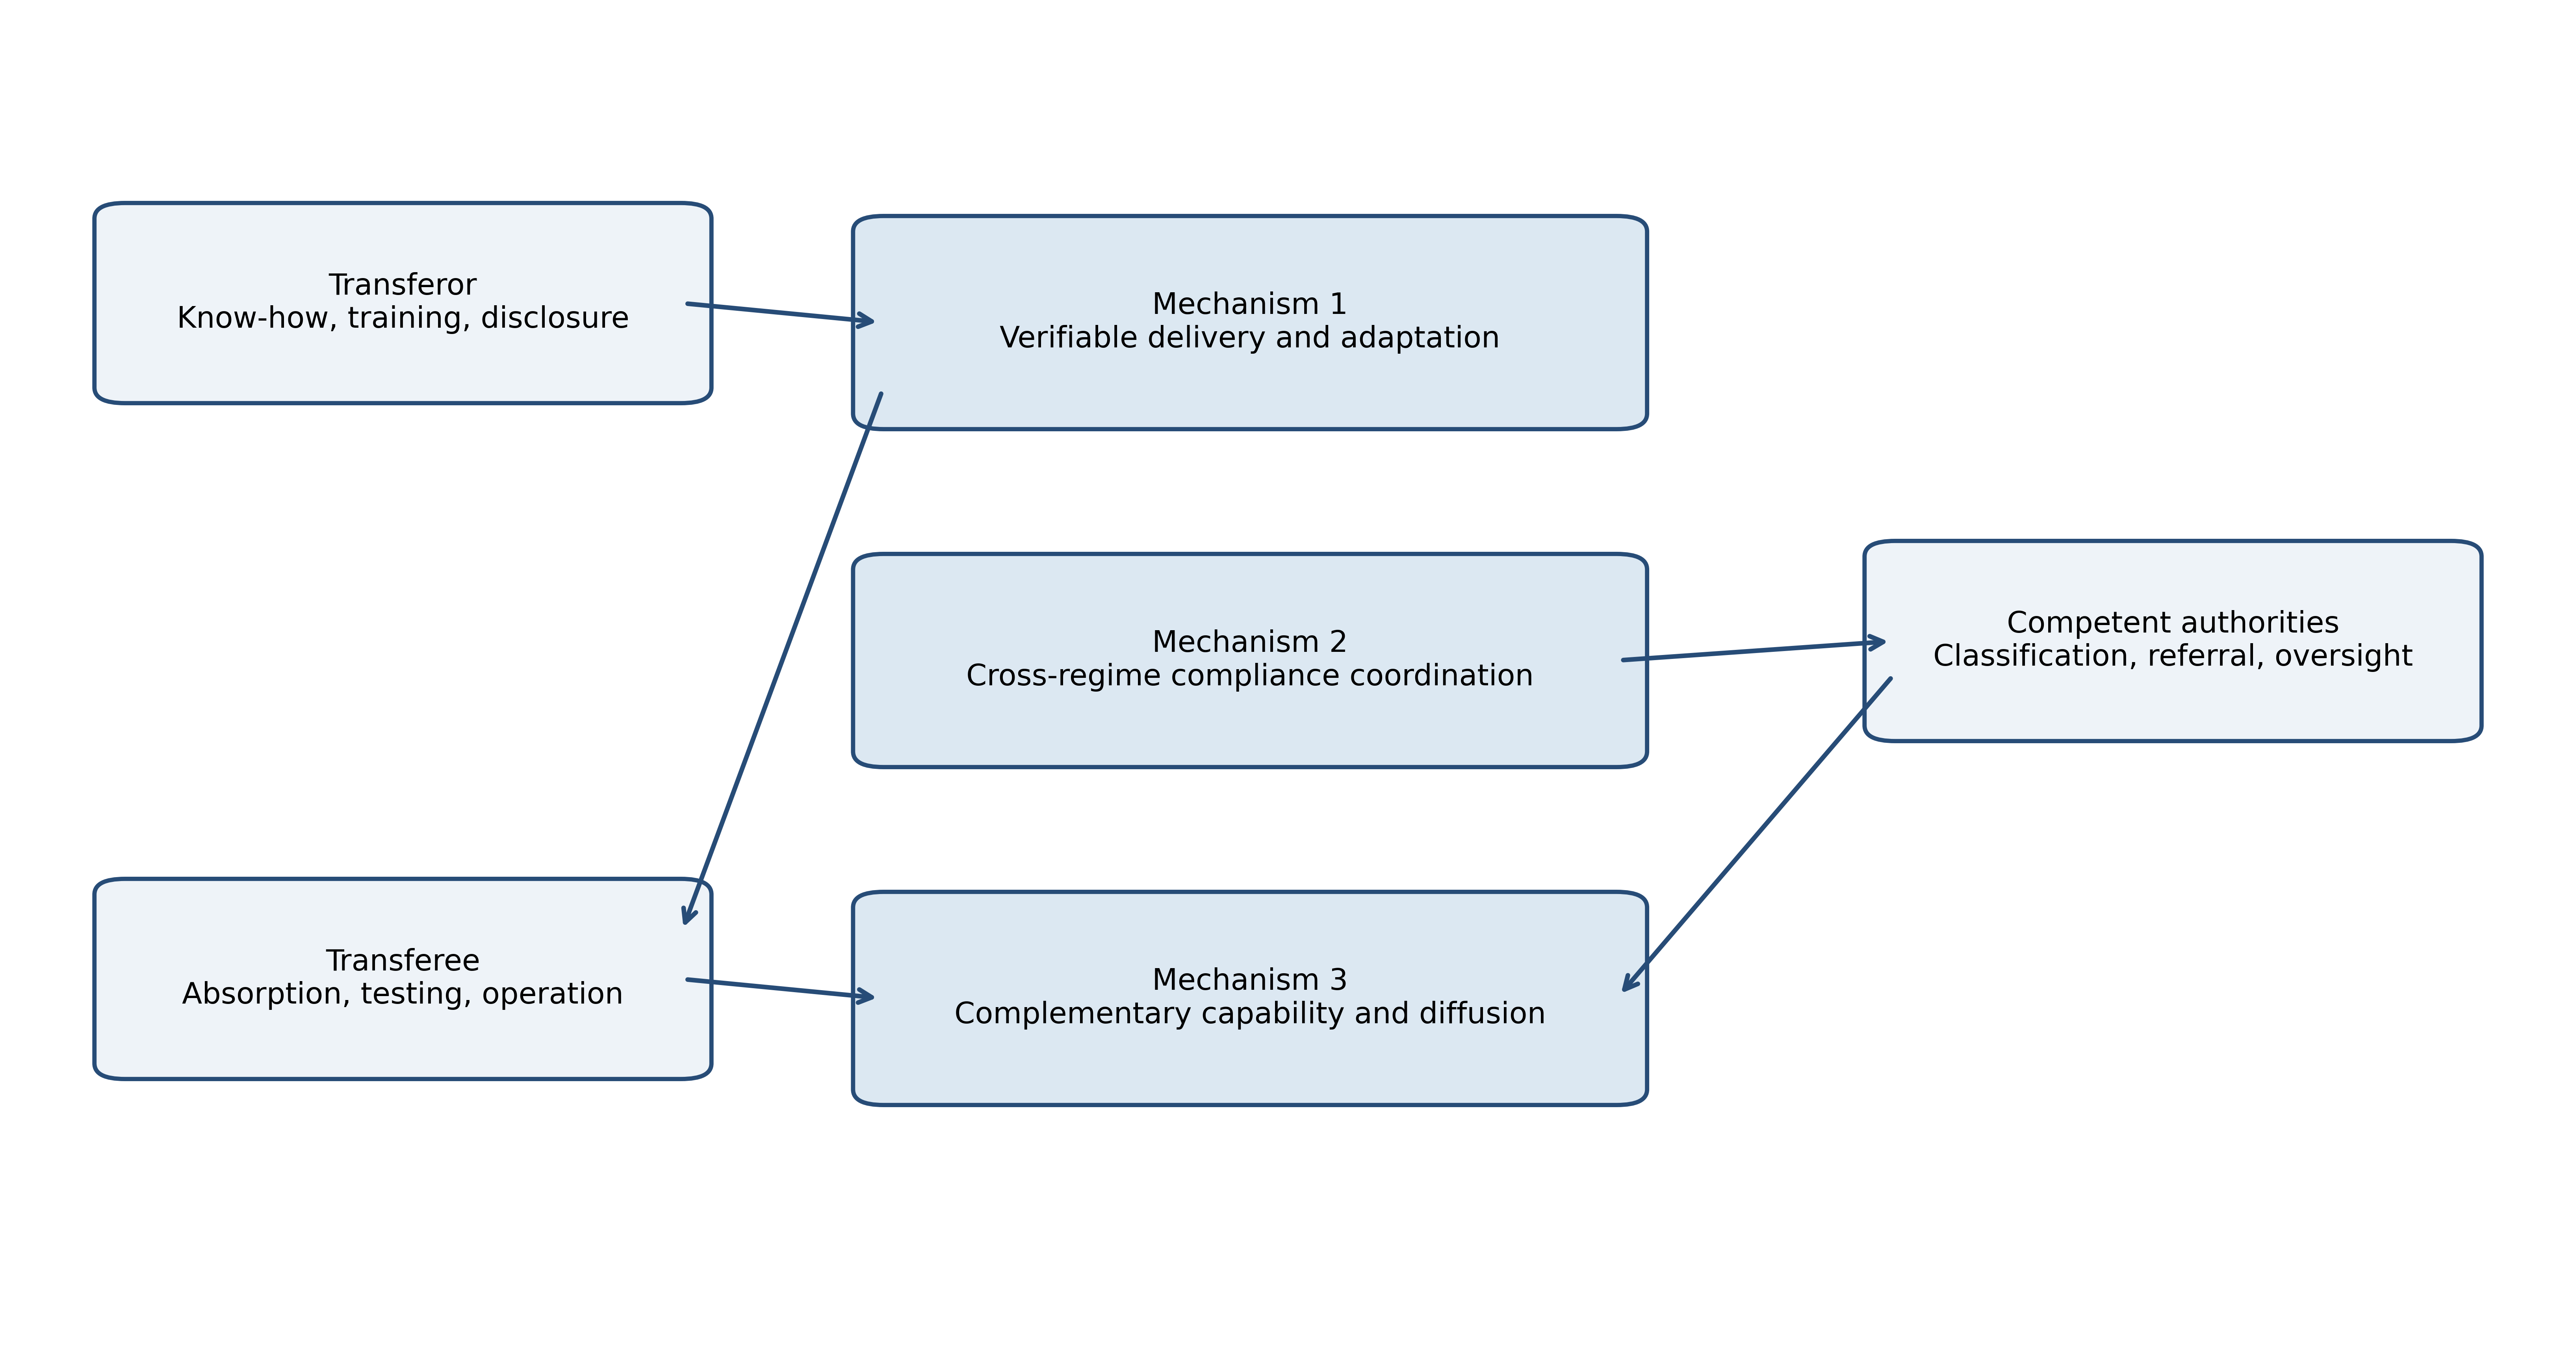
\includegraphics[width=6.2in,height=3.2422in]{figures/Fig3_Mechanism_Map.png}

\emph{Fig. 3 Mechanisms connecting transaction actors, regulators and
transfer performance}

\section{5 A dual-function framework for regulatory
resilience}\label{a-dual-function-framework-for-regulatory-resilience}

The findings support a dual-function account of the transfer contract.
Function 1 is private performance: the contract identifies the
technology, links delivery to acceptance, organises training and
corrective work, allocates adaptation and improvement rights, and
connects observable milestones to payment and warranty. Function 2 is
compliance coordination: the contract records the
parties\textquotesingle{} regulatory roles, lawful bases for data and
know-how access, information duties, security responsibilities and
procedures for regulatory engagement.

These functions are connected but not merged. A contract cannot confer
ownership that the law does not recognise, authorise unlawful
disclosure, bind an authority or transfer a public power. Nor does
administrative registration constitute technical acceptance or
commercial viability. The framework instead asks whether information
produced for performance can be reused lawfully to make regulatory
interfaces intelligible and whether regulatory decisions arrive early
enough to permit adaptation.

Table 3 maps ten recurrent questions to the principal legal route. Its
categories avoid two opposite errors: treating every referral as a gap
and treating the existence of any rule as proof of an effective
connection. Transfer-framework rules operate within the dedicated
statute; distributed or conditional protection depends on another regime
or eligibility condition; an open default-design question identifies the
absence of a technology-specific default for the precise function
reviewed without excluding general law. Table 4 then compares four
functions across selected international instruments. The comparison is
diagnostic rather than a claim of legal equivalence: it identifies the
design question that each comparator makes visible for Vietnam.

For state management, the proposal is a time-limited coordination pilot
rather than a new general approval. A single contact would triage a case
and route defined questions to relevant competent bodies. Each body
would retain its statutory authority. A protected case record would
identify contacts, legal bases, status, reasons and review routes.
Scheduled review would examine unresolved referrals alongside
acceptance, training and operating capability.

The pilot must be tested for costs as well as benefits. It could reduce
repeated information requests and late classification changes, or create
another bottleneck. Confidential know-how and personal data must not
become generally accessible. Smaller firms must be able to use the
process, referrals must remain contestable, and service targets must not
displace statutory time limits or substantive tests. Figure 4 states
these safeguards as part of the design rather than benefits assumed to
follow from a portal.

{\def\LTcaptype{none} % do not increment counter
\begin{longtable}[]{@{}
  >{\raggedright\arraybackslash}p{(\linewidth - 4\tabcolsep) * \real{0.3333}}
  >{\raggedright\arraybackslash}p{(\linewidth - 4\tabcolsep) * \real{0.3333}}
  >{\raggedright\arraybackslash}p{(\linewidth - 4\tabcolsep) * \real{0.3333}}@{}}
\toprule\noalign{}
\begin{minipage}[b]{\linewidth}\centering
\textbf{Question}
\end{minipage} & \begin{minipage}[b]{\linewidth}\centering
\textbf{Principal legal route}
\end{minipage} & \begin{minipage}[b]{\linewidth}\centering
\textbf{Classification}
\end{minipage} \\
\midrule\noalign{}
\endhead
\bottomrule\noalign{}
\endlastfoot
Contract contents and transfer modes & Law on Technology Transfer arts
6, 22--23 & Transfer-framework rule \\
Price and payment & Law art 27; Decree 101/2026 art 18 &
Transfer-framework rule \\
Restrictive licence terms & IP Law art 144; Competition Law arts 11--14,
24--27 & Conditional protection \\
Delivery, acceptance and warranty linkage & Contract terms plus
applicable general law & Open tailored-default question \\
Digital transfers and downstream AI duties & Decree 101; Data Law; AI
Law & Distributed, transaction-specific \\
Semiconductor capability & Digital Technology Industry Law ch III; High
Technology Law & Distributed regulation \\
Semiconductor compulsory licensing & IP Law art 146(1)(b); TRIPS art
31(c) & Treaty-constrained protection \\
State-funded research results & Science, Technology and Innovation Law
arts 24--28 & Distributed regulation \\
Agricultural diffusion & Law on Technology Transfer art 52(5) &
Administrative transfer channel \\
Private-transfer valuation & Agreement; Decree 101; valuation standards
& Framework plus capability question \\
\end{longtable}
}

\emph{Table 3 Selected regulatory interfaces around a
technology-transfer relationship}

{\def\LTcaptype{none} % do not increment counter
\begin{longtable}[]{@{}
  >{\raggedright\arraybackslash}p{(\linewidth - 6\tabcolsep) * \real{0.2500}}
  >{\raggedright\arraybackslash}p{(\linewidth - 6\tabcolsep) * \real{0.2500}}
  >{\raggedright\arraybackslash}p{(\linewidth - 6\tabcolsep) * \real{0.2500}}
  >{\raggedright\arraybackslash}p{(\linewidth - 6\tabcolsep) * \real{0.2500}}@{}}
\toprule\noalign{}
\begin{minipage}[b]{\linewidth}\centering
\textbf{Function}
\end{minipage} & \begin{minipage}[b]{\linewidth}\centering
\textbf{Selected comparator}
\end{minipage} & \begin{minipage}[b]{\linewidth}\centering
\textbf{Vietnamese position}
\end{minipage} & \begin{minipage}[b]{\linewidth}\centering
\textbf{Design implication}
\end{minipage} \\
\midrule\noalign{}
\endhead
\bottomrule\noalign{}
\endlastfoot
Adaptive performance & US/EU contract law and licensing guidance leave
delivery architecture mainly to agreement & Dedicated contract chapter
lists contents, price, warranty and liability; no technology-specific
acceptance sequence & Tie tests, corrective work, payment and warranty
to observable milestones \\
Restrictive licensing & EU TTBER/guidelines and US licensing guidance
distinguish efficiency-supporting restraints from foreclosure & IP Law
art 144 and Competition Law provide conditional, distributed controls &
Screen grant-backs, sourcing, territory and improvements under both
regimes \\
Data and AI transfer & EU Data Act regulates defined access; EU AI Act
allocates provider and downstream duties & Transfer law recognises data,
software, models and algorithms; Data and AI Laws govern separate
functions & Specify lawful access, permitted use, disclosure, records,
incidents and role changes \\
Semiconductor capability & US CHIPS Act and EU Chips Act emphasise
finance, facilities, pilot lines and skills & Sectoral incentives and
strategic-technology rules coexist with treaty-constrained compulsory
licensing & Combine voluntary licences with training, facilities and
transparent access terms \\
\end{longtable}
}

\emph{Table 4 Functional international comparison and design
implications}

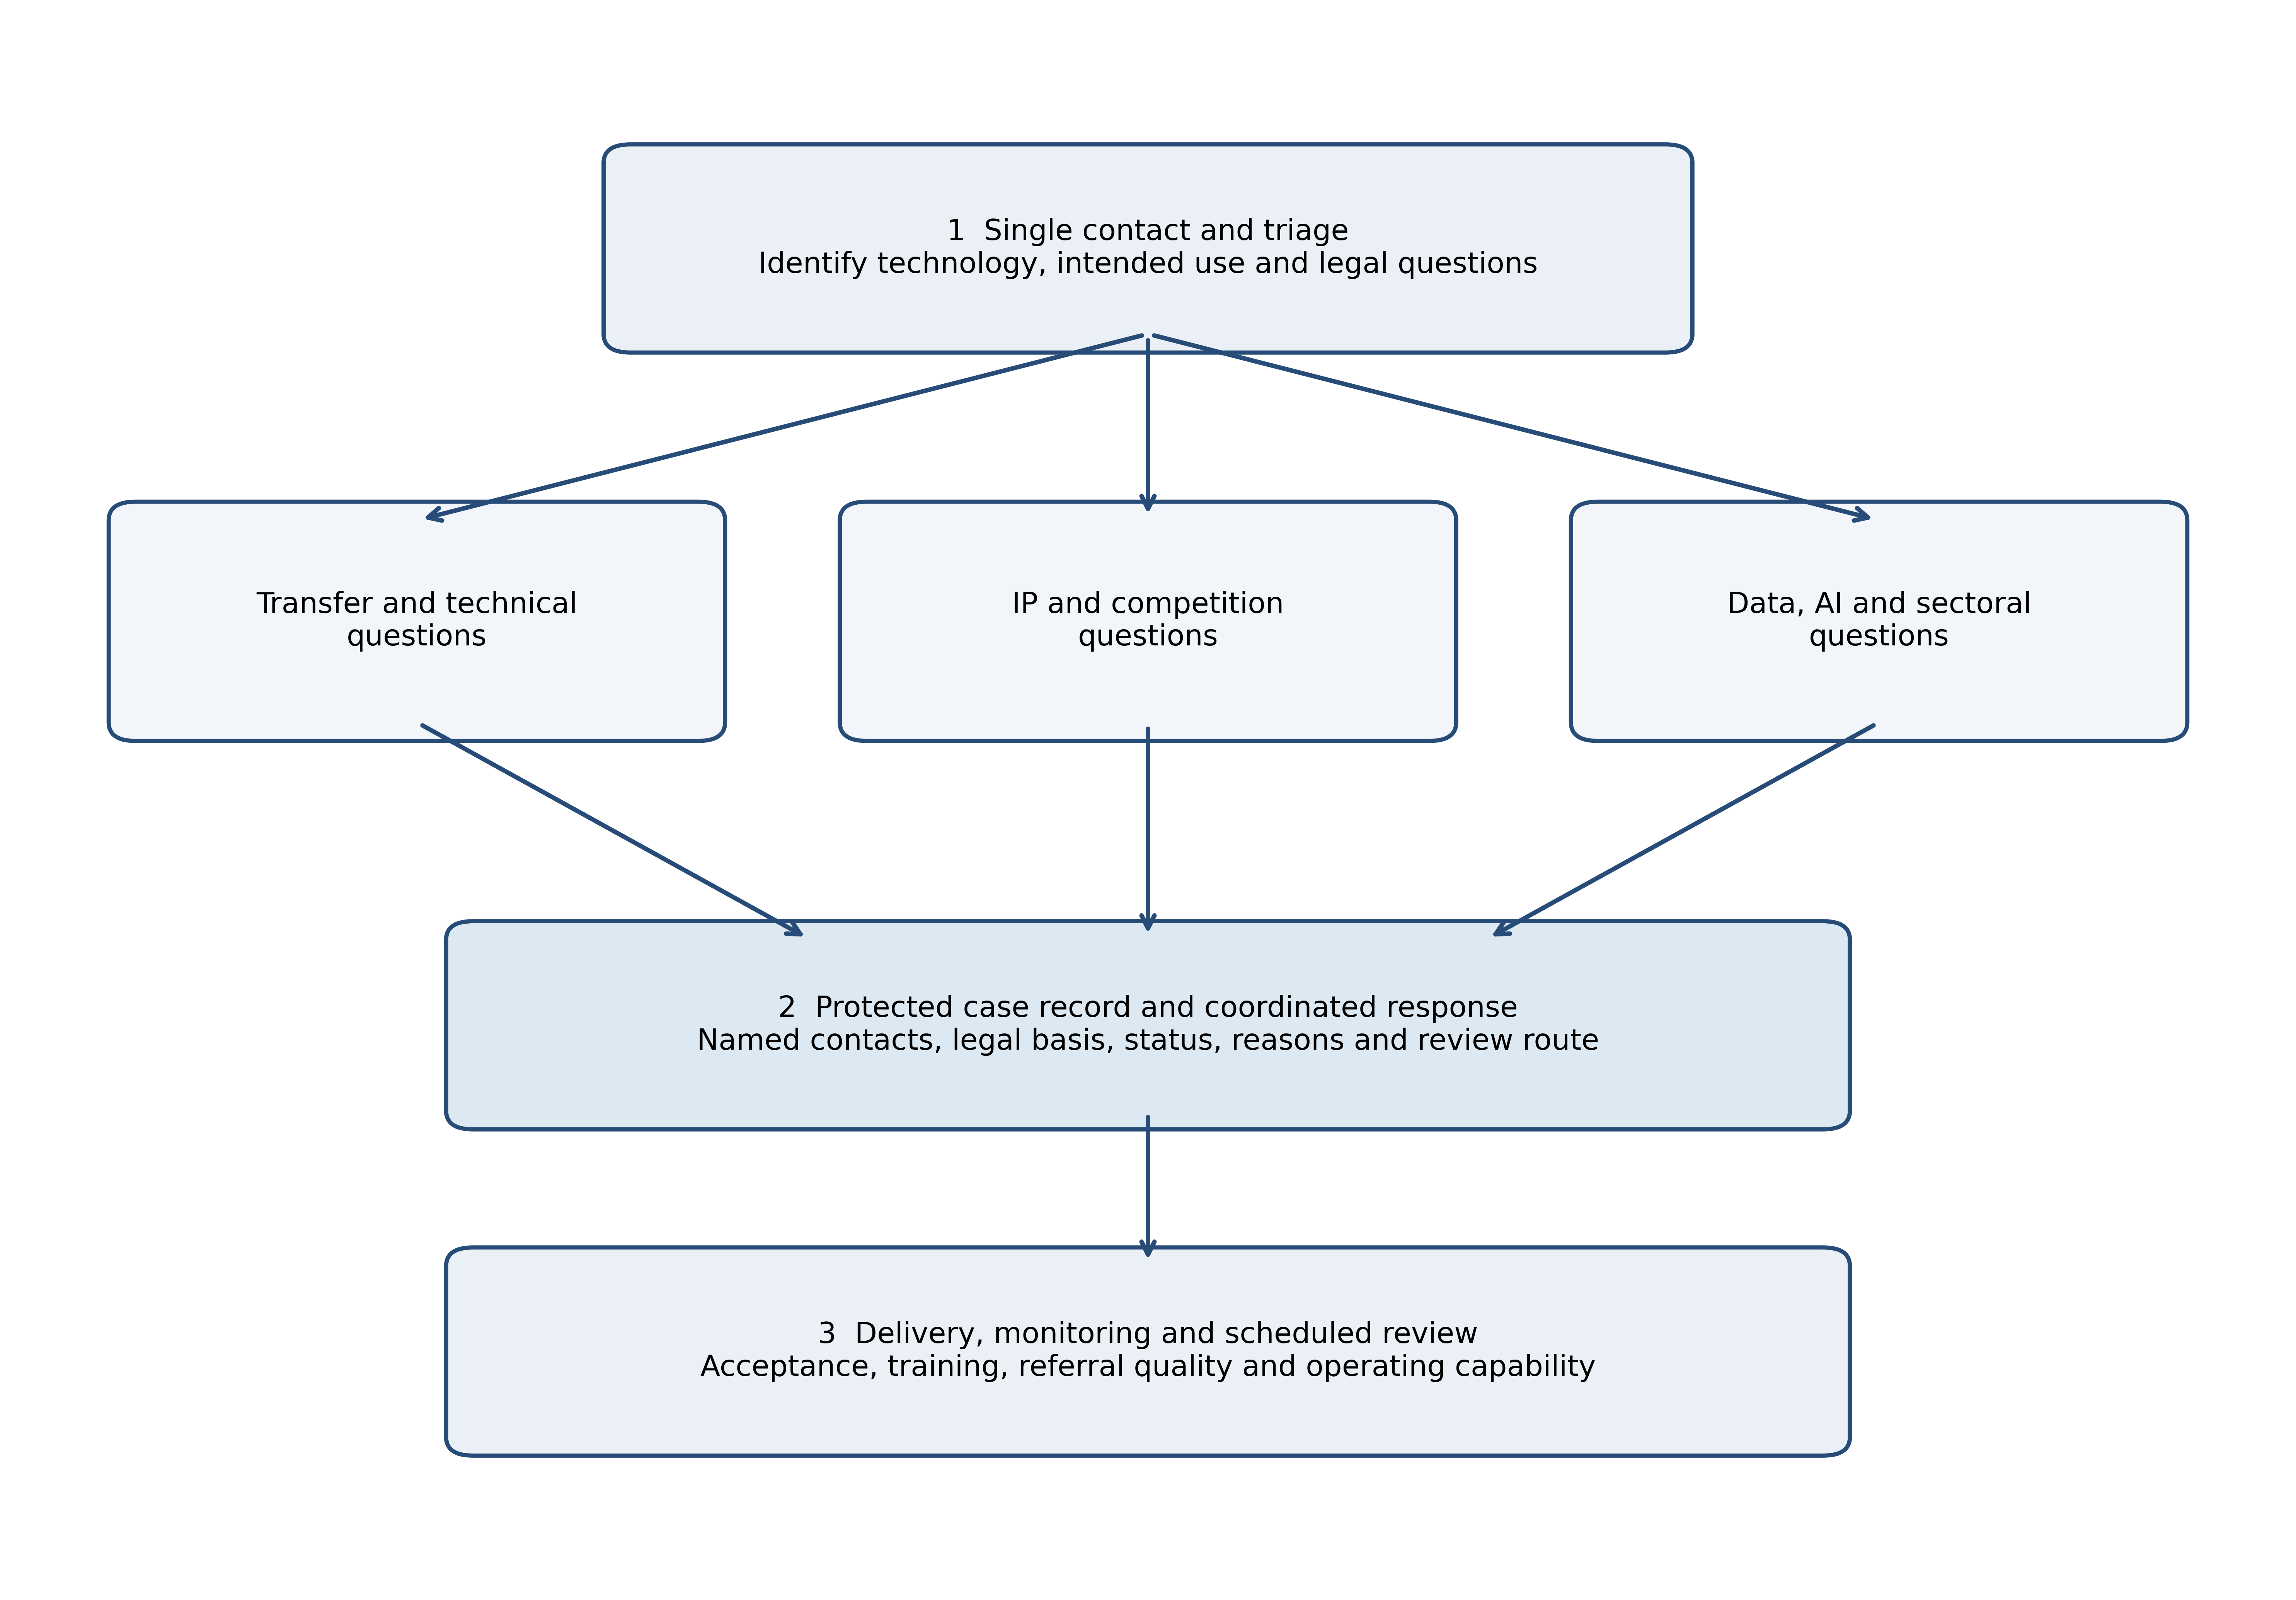
\includegraphics[width=5.1in,height=3.55455in]{figures/Fig4_Coordination_Pilot.png}

\emph{Fig. 4 Proposed coordination pilot. It is not an existing
procedure or a single approval route}

\section{6 Discussion and testable
implications}\label{discussion-and-testable-implications}

The study\textquotesingle s broader claim is that regulatory resilience
depends on usable connections among specialised functions. Multiple
statutes are not inherently dysfunctional. Fragmentation becomes an
empirical condition when participants cannot identify responsibilities,
relevant decisions arrive too late for performance, information must be
repeatedly reconstructed, or authorities apply incompatible
classifications without a reviewable route. This definition permits
comparison across jurisdictions without treating an emerging-economy
label as an explanation.

The framework yields two propositions. First, if uncertainty about
delivery is consequential, otherwise comparable transfers with explicit
performance tests, correction procedures and payment milestones should
exhibit fewer unresolved delivery disputes than transfers relying on
generic descriptions. Second, if coordination is consequential, projects
receiving earlier and reasoned referral among relevant authorities
should experience fewer repeated compliance requests and late
classification changes.

These propositions require data not available in the current corpus:
contract files, acceptance records, administrative correspondence,
judgments and interviews. Well-resourced parties may both draft better
contracts and complete transfers more successfully. Complex technologies
may generate more referrals and disputes regardless of administrative
quality. Cases in which general law resolves a dispute despite sparse
technology-specific drafting, or extensive contractual detail fails to
prevent breakdown, are essential contrary cases.

The capability mechanism supplies an additional rival explanation.
Finance, skills, facilities and organisational incentives may remain
binding even when legal guidance is clear. Evaluation should therefore
separate processing measures from operating outcomes. Referral time and
repeated requests are coordination indicators; acceptance, training
completion and the recipient\textquotesingle s capacity to operate the
technology are performance indicators. Neither alone establishes
economic or social value.

The Vietnamese case is analytically transferable where three conditions
recur: performance depends on continuing cooperation, the transaction
crosses regulatory mandates, and implementation depends on complementary
public or organisational capacity. The particular clauses, agencies and
statutory boundaries will differ. Transferability lies in the questions
and mechanisms, not in copying Vietnam\textquotesingle s legal
architecture or assuming that all emerging economies share its
constraints.

The research design also offers a methodological lesson. A small
mixed-genre corpus can make agenda-setting transparent, but it cannot
convert published argument into representative evidence. Sensitivity to
genre is a substantive result because it shows which questions are
carried by legal scholarship rather than public reporting. The correct
response is to qualify the inference and connect it to doctrinal
analysis, not to claim that model agreement validates a legal
conclusion.

\section{7 Conclusion}\label{conclusion}

Technology-transfer systems must do more than define transferable
objects and allocate rights. They must help a continuing relationship
reach demonstrable operating capability while preserving the distinct
mandates that govern intellectual property, competition, data,
artificial intelligence and sectoral risk. Vietnam\textquotesingle s
recent reforms provide extensive distributed and conditional protection,
but they leave important connective functions to contractual design and
administrative practice.

The article\textquotesingle s principal contribution is a dual-function
account of the transfer contract. The contract is both a private
performance arrangement and a compliance protocol. The two functions may
rely on shared records and responsibilities, but their legal effects
remain separate: private agreement cannot alter public powers or
mandatory duties. A time-limited coordination pilot provides a way to
test whether this connective role reduces duplication and late
classification without creating another approval layer.

Three mechanisms organise the findings. Verifiable delivery links
acceptance, correction, payment and warranty. Cross-regime coordination
distinguishes transferability from ownership, lawful access and
downstream compliance. Complementary capability explains why licences
and definitions cannot substitute for skills, facilities, finance,
extension institutions or valuation expertise. These mechanisms suggest
different interventions and prevent legal-design problems from being
conflated with implementation failure.

The limitations are substantial. Thirty-four publications cannot
establish prevalence, causation or institutional performance. The
contract-law grouping is small and genre-dependent. The study does not
examine transaction files or evaluate the pilot. Its contribution is a
bounded legal map, a mechanism-based framework and an empirical research
programme. Subsequent work should test the propositions against
contracts, acceptance records, administrative correspondence and
judgments after the 2025--2026 reforms.

The legal map is current to 1 October 2026. Future use must check
commencement provisions, implementing instruments and
transaction-specific scope. That discipline is part of the
article\textquotesingle s substantive point: regulatory resilience
depends not only on the existence of rules, but on accurate, timely and
usable connections among them.

\section{Data availability}\label{data-availability}

An anonymized replication package is supplied as Supplementary
Information. It contains the corpus inventory, supplementary model
settings, scripts, document-topic assignments, K-scan outputs and
robustness summaries used for the sensitivity audit and Fig. S1.
Copyrighted full texts are not redistributed. The public repository URL
is provided to the editor in the title-page and cover-letter files and
will be inserted in the manuscript after anonymous review.

\section{Legal and policy
instruments}\label{legal-and-policy-instruments}

European Commission (2026). Commission Regulation (EU) 2026/877 of 16
April 2026 on categories of technology transfer agreements; Guidelines
on Article 101 TFEU technology transfer agreements.

European Parliament and Council (2023). Regulation (EU) 2023/1781
(European Chips Act); Regulation (EU) 2023/2854 (Data Act).

European Parliament and Council (2024). Regulation (EU) 2024/1689
(Artificial Intelligence Act).

Government of Vietnam (2026). Decree No. 101/2026/NĐ-CP detailing the
Law on Technology Transfer.

Ministry of Finance of Vietnam (2024). Circular No. 37/2024/TT-BTC on
valuation of intangible assets.

National Assembly of Vietnam (2005). Commercial Law No. 36/2005/QH11;
Intellectual Property Law No. 50/2005/QH11, as amended.

National Assembly of Vietnam (2015). Civil Code No. 91/2015/QH13.

National Assembly of Vietnam (2017). Law on Technology Transfer No.
07/2017/QH14, as amended through Law No. 115/2025/QH15.

National Assembly of Vietnam (2018). Competition Law No. 23/2018/QH14.

National Assembly of Vietnam (2023). Prices Law No. 16/2023/QH15, as
amended.

National Assembly of Vietnam (2024). Data Law No. 60/2024/QH15.

National Assembly of Vietnam (2025). Artificial Intelligence Law No.
134/2025/QH15; Digital Technology Industry Law No. 71/2025/QH15; High
Technology Law No. 133/2025/QH15; Law on Science, Technology and
Innovation No. 93/2025/QH15.

National Assembly of Vietnam (2026). Law No. 20/2026/QH16 amending,
inter alia, the Law on Technology Transfer.

Office of the National Assembly of Vietnam (2026). Consolidated Text of
the Law on Technology Transfer No. 138/2026/VBHN-LQ-VPQH.

Prime Minister of Vietnam (2026). Decision No. 21/2026/QĐ-TTg on
strategic technologies and products.

United States Congress (2022). CHIPS and Science Act, Public Law
117-167.

United States Department of Justice and Federal Trade Commission (2017).
Antitrust Guidelines for the Licensing of Intellectual Property.

World Trade Organization (1994). Agreement on Trade-Related Aspects of
Intellectual Property Rights, arts 31(c) and 40.

\section{References}\label{references}

Abid, N., Cunningham, J. A., \& Perea-Vicente, J.-L. (2025). A thematic
review of 45 years of The Journal of Technology Transfer. The Journal of
Technology Transfer, 50, 1739--1784.
https://doi.org/10.1007/s10961-024-10154-x

Bozeman, B. (2000). Technology transfer and public policy: A review of
research and theory. Research Policy, 29(4--5), 627--655.

Bozeman, B., Rimes, H., \& Youtie, J. (2015). The evolving
state-of-the-art in technology transfer research. Research Policy,
44(1), 34--49.

Bradley, S. R., Hayter, C. S., \& Link, A. N. (2013). Models and methods
of university technology transfer. Foundations and Trends in
Entrepreneurship, 9(6), 571--650.

Bùi Thị Hằng Nga. (2019). Học thuyết điều kiện thiết yếu và nghĩa vụ
chuyển giao quyền sở hữu trí tuệ theo quy định của pháp luật cạnh tranh.
Tạp chí Nghiên cứu Lập pháp, 13(389).

Drexl, J. (2017). Designing competitive markets for industrial
data---Between propertisation and access. JIPITEC, 8(4), 257--292.

Đỗ Văn Đại. (2022). Luật hợp đồng Việt Nam---Bản án và bình luận bản án.
NXB Hồng Đức.

Cao, Z., \& Lumineau, F. (2015). Revisiting the interplay between
contractual and relational governance: A qualitative and meta-analytic
investigation. Journal of Operations Management, 33--34, 15--42.
\url{https://doi.org/10.1016/j.jom.2014.09.009}

Cunningham, J. A., Menter, M., \& Starke, F. (2025). The evolution of
university technology transfer research: A text mining approach. The
Journal of Technology Transfer, 50, 1231--1268.
https://doi.org/10.1007/s10961-024-10133-2

Fuglie, K., Gautam, M., Goyal, A., \& Maloney, W. F. (2020). Harvesting
prosperity: Technology and productivity growth in agriculture. World
Bank.

Gilson, R. J., Sabel, C. F., \& Scott, R. E. (2009). Contracting for
innovation. Columbia Law Review, 109(3), 431--502.

Grindley, P. C., \& Teece, D. J. (1997). Managing intellectual capital:
Licensing and cross-licensing in semiconductors and electronics.
California Management Review, 39(2), 8--41.

Hồ Minh Khánh. (2024). Đánh giá thực trạng quy định pháp luật Việt Nam
về hợp đồng chuyển giao công nghệ. Tạp chí Quản lý Nhà nước.

Kamiyama, S., Sheehan, J., \& Martinez, C. (2006). Valuation and
exploitation of intellectual property. OECD STI Working Papers 2006/05.

Lemley, M. A., \& Casey, B. (2021). Fair learning. Texas Law Review,
99(4), 743--785.

Lodge, M., \& Wegrich, K. (Eds.). (2014). The problem-solving capacity
of the modern state. Oxford University Press.

Macaulay, S. (1963). Non-contractual relations in business: A
preliminary study. American Sociological Review, 28(1), 55--67.

Macneil, I. R. (1980). The new social contract: An inquiry into modern
contractual relations. Yale University Press.

Nguyễn Thị Minh Phương, \& Phí Công Thường. (2026). Định giá, thẩm định
giá tài sản trí tuệ: Những vấn đề pháp lý và thực tiễn tại Việt Nam. Tạp
chí Khoa học và Công nghệ Việt Nam.

Phạm Chí Trung. (2016). Một số nội dung cần sửa đổi, bổ sung của Luật
Chuyển giao công nghệ năm 2006. Tạp chí Nghiên cứu Lập pháp.

Phan Quoc Nguyen. (2020). Legal rules on university technology transfer
from a comparative perspective between Vietnam and the USA. US-China Law
Review, 17(2).

Phan Quoc Nguyen, \& To Nhat Mai. (2024). Legal rules on patent
exploitation and management for innovation in Vietnamese universities.
Edelweiss Applied Science and Technology, 8(6).

Perkmann, M., Salandra, R., Tartari, V., McKelvey, M., \& Hughes, A.
(2021). Academic engagement: A review of the literature 2011--2019.
Research Policy, 50(1), 104114.
https://doi.org/10.1016/j.respol.2020.104114

Phùng Minh Hải. (2026). Thương mại hóa sáng chế từ viện nghiên cứu,
trường đại học. Tạp chí Khoa học và Công nghệ Việt Nam, 4A.

Samuelson, P. (2023). Generative AI meets copyright. Science, 381(6654),
158--161.

Teece, D. J. (1986). Profiting from technological innovation. Research
Policy, 15(6), 285--305.

Williamson, O. E. (1979). Transaction-cost economics: The governance of
contractual relations. Journal of Law and Economics, 22(2), 233--261.

\end{document}
